\chapter{Contribution}

The main contribution of this thesis is an active automaton learning framework, which can be used to support system design and analysis. This framework, since used in system engineering, is required to be easily modifiable and extensible, while having the capability of handling any variation of formalisms systems might rely on.


\section{Automaton learning framework}

Active automaton learning algorithms essentially have two endpoints: the input, reached through the teacher component, and the output, where the learned hypothesis automaton is returned. This is illustrated in Fig. \ref{fig:learningcomm}. The teacher and the learner can be adjusted to the required formalisms: the underlying modeling language of the system under learning (the \emph{input formalism}) and that of the learned hypothesis (the \emph{output formalism}). \\
\begin{figure}[H]
	\centering
	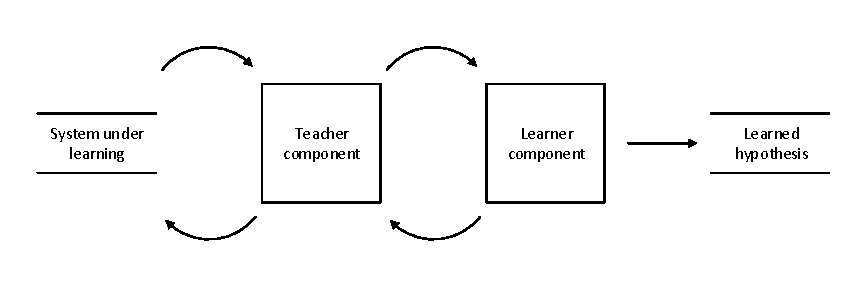
\includegraphics[width=1.0\linewidth]{figures/learningcomm}
	\caption{Data flow of active learning algorithms.}
	\label{fig:learningcomm}
\end{figure}

\subsection{Tooling}

As seen in Fig. \ref{fig:learningcomm}, the variables of the framework are essentially the input and output formalisms it accepts. In order to provide flexibility in this regard, the following tools were used.

\begin{itemize}
	\item \textbf{Eclipse Modeling Framework (EMF):} EMF, or more specifically, EMF core, is an "abstraction for describing, composing, and manipulating structured information", essentially a tool for system modeling and code generation implemented in Java. The tool it provides allows graphical modeling of UML class diagrams and generating code based on these models.
	\item \textbf{Xtext:} Xtext is a framework for creating programming and domain-specific languages, which also has integration with EMF. This integration allows reading and writing text files in the form of an Xtext grammar using corresponding EMF generated classes.
\end{itemize}


\subsection{High-level overview}

Since the implementation of the framework would be using Java as a language, the high-level view seen in Fig. \ref{fig:abstractoverview} is an UML class diagram of the packages and the relations between them, essentially being an overview of the modularization of the framework.

\begin{figure}
	\centering
	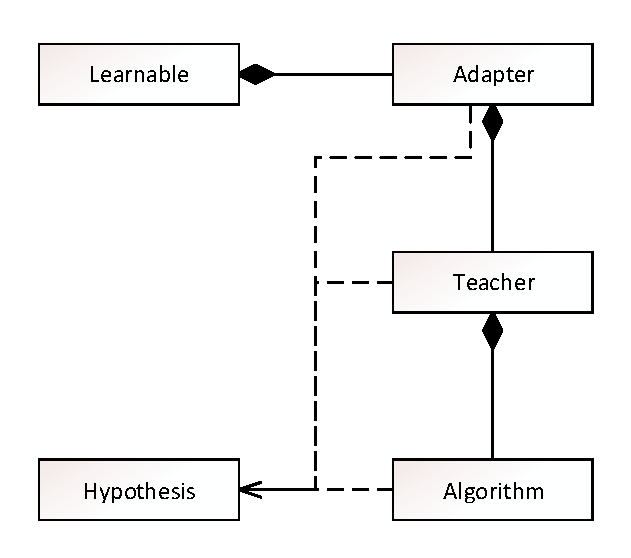
\includegraphics[width=0.5\linewidth]{figures/abstractoverview}
	\caption{Structure and relations of the packages comprising the framework.}
	\label{fig:abstractoverview}
\end{figure}

Note, that when comparing Fig. \ref{fig:abstractoverview} to Fig. \ref{fig:learningcomm}, the data flows identically. The Learnable package containing the input formalisms, and the Hypothesis package containing the output formalisms are used by the teacher (Teacher package) and the learner (Algorithm package). The package not represented on Fig. \ref{fig:learningcomm}, the Adapter package is used as an abstraction layer to separate the algorithm and the teacher from the input formalism. Since automaton learning algorithms have no direct access to the system under learning, they operate in a black-box way, the Adapter package is a useful addition. Unfortunately no such adapter can be used on the output layer, since Hypotheses are directly accessed by the learning algorithms, and are constructed during the learning. While more specific abstractions were made (and can be seen later), no singular abstraction layer can be provided for every type of automaton and every type of learning algorithm the same way as for the input formalisms.
\\\\
The relations between the packages (modules) are straightforward. Composition is used, to indicate, that there is no Algorithm (learner) without a Teacher, there is no Teacher without an Adapter, and there is no Adapter without an input, a Learnable, to adapt. Algorithms of course depend on Hypothesis, and because of equivalence queries, which are later transferred through the Teacher and Adapter components, they both also have a dependency on the Hypothesis package.

\subsection{Detailed overview of abstractions}


The diagram in Figure \ref{fig:abstractoverview} showed the modularization of the framework, which depend on the correct implementation of object-oriented architecture so the notated compositions and dependencies in Fig. \ref{fig:abstractoverview} are satisfied. These abstractions are defined and implemented in Java as abstract classes and interfaces seen in Fig. \ref{fig:abstractdetailedoverview}. The detailed descriptions of these abstractions are as follows.
\\
\begin{itemize}
	\item \textbf{Learnable:} The \emph{Learnable} interface is the input type used by the framework. It defines two generic parameters, \emph{I} is the character type of the regular language the Learnable represents, while \emph{O} is the character type by which actions are defined for the system under learning. The only method the interface defines is the \emph{getOutput()} method, which returns the output \emph{O} given by the system under learning for a specific sequence of inputs. Note, that while the word "output" is used, the \emph{O} it returns is the action the system takes for an input. If the system is represented as a DFA, this would be the state it moves to, if the system is represented as a Mealy machine, it would be an output.
	
	\item \textbf{Hypothesis:} The \emph{Hypothesis} interface is the output type used by the framework. The generic parameters it takes are the automaton it uses (\emph{M}), and the input (\emph{I}), output (\emph{O}), state (\emph{S}) and transition (\emph{T}) types used by \emph{M}. The Hypothesis class does not enforce bounds on these parameters to allow flexibility in implementation. Beyond the getters, the \emph{query()} method takes a sequence of inputs, and returns the output given by the hypothesis automaton. Just as with the \emph{Learnable} interface, this output represents action in the automaton.
	
	\item \textbf{LearnableAdapter:} The \emph{LearnableAdapter} abstract class is the abstraction of the adaptation between any \emph{Learnables} and \emph{Hypotheses}. The generic parameters of it are the \emph{Hypothesis} type (\emph{H}) and the input, output types of \emph{H} (\emph{HI}, \emph{HO}), similarly, the \emph{Learnable} type (\emph{L}) and the input, output types of \emph{L} (\emph{LI}, \emph{LO}). The \emph{LearnableAdapter} class stores a \emph{Learnable}, the object which represents the data of the system under learning. It gives access to the system using the \emph{membershipQuery()} method and the abstract \emph{equivalenceQuery()} method. The abstract \emph{covert..()} methods are used to do the actual adapting between \emph{Hypotheses} and \emph{Learnables} character by character.
	
	\item \textbf{Teacher:} The \emph{Teacher} abstract class defines the "middle ground" between a learning algorithm and the input. The \emph{Teacher} class as generic parameter, takes a \emph{Hypothesis} (\emph{H}) with input and outputs types of \emph{HI} and \emph{HO}, also a \emph{LearnableAdapter} (\emph{LA}) which has the same \emph{Hypothesis} type as \emph{H}. It defines two query types, \emph{membershipQuery()} and \emph{equivalenceQuery}, both of which it delegates to the current adapter object in its adapter field. The \emph{Teacher class} is needed for easy extensibility, specifically, for any algorithm and input to work together without modification on them.
	
	\item \textbf{ActiveLearningAlgorithm:} The \emph{ActiveLearningAlgorithm} class provides abstraction for active automaton learning algorithms. It defines only a \emph{Hypothesis}  (\emph{H}), and its input types (\emph{HI}, \emph{HO}). The teacher field bounded to the \emph{Hypothesis} \emph{H} is used for queries, while the \emph{execute()} method executes the algorithm and returns with the learned \emph{Hypothesis}. Note, that the algorithm is fully separated from the system it is learning, it does not even know the generic type which with the communication, queries are executed.
\end{itemize}


\begin{figure}[H]
	\centering
	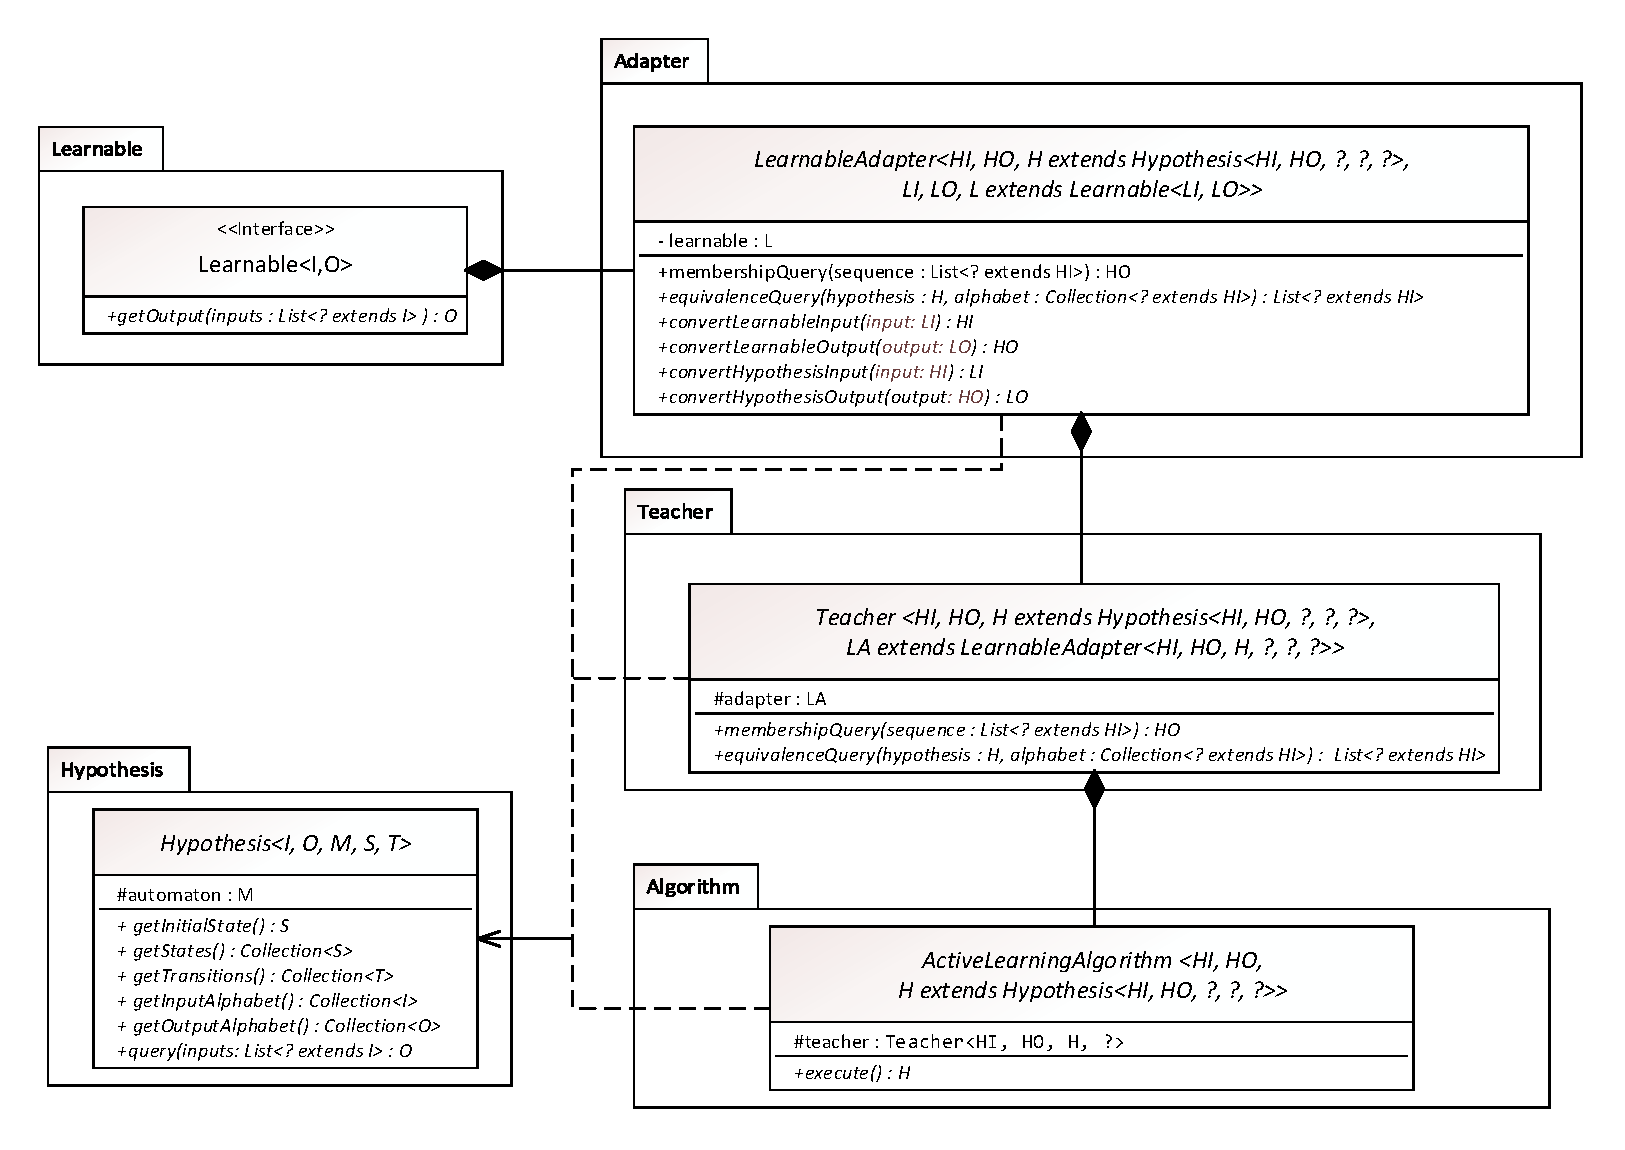
\includegraphics[width=0.97\linewidth]{figures/abstractdetailedoverview}
	\caption{Overview of the abstract classes and interfaces of the framework.}
	\label{fig:abstractdetailedoverview}
\end{figure}

\section{Implemented learning algorithms}

Building upon the abstractions of the framework, I implemented the two active learning algorithms presented in the Background chapter. The first step of the implementation was determining the input and output formalisms to use.

Since automaton learning algorithms can be implemented on any type of automata, the easiest method would be using deterministic finite automata. However, real-life reactive systems usually are better modeled using Mealy machines, hence the implementation was made using Mealy machines as both input and output formalisms.
\\
The first step of the implementation process was choosing the right tooling, which is why the Mealy machine implementation was done in Eclipse Modeling Framework.
\\\\
Figure \ref*{fig:mealyecore} shows an UML class diagram of the metamodel I've created using the Ecore package of EMF core, and the graphical modeling tool provided by EMF. I also used EMF to generate Java classes corresponding to the ones seen in Fig. \ref*{fig:mealyecore}.

\begin{figure}
	\centering
	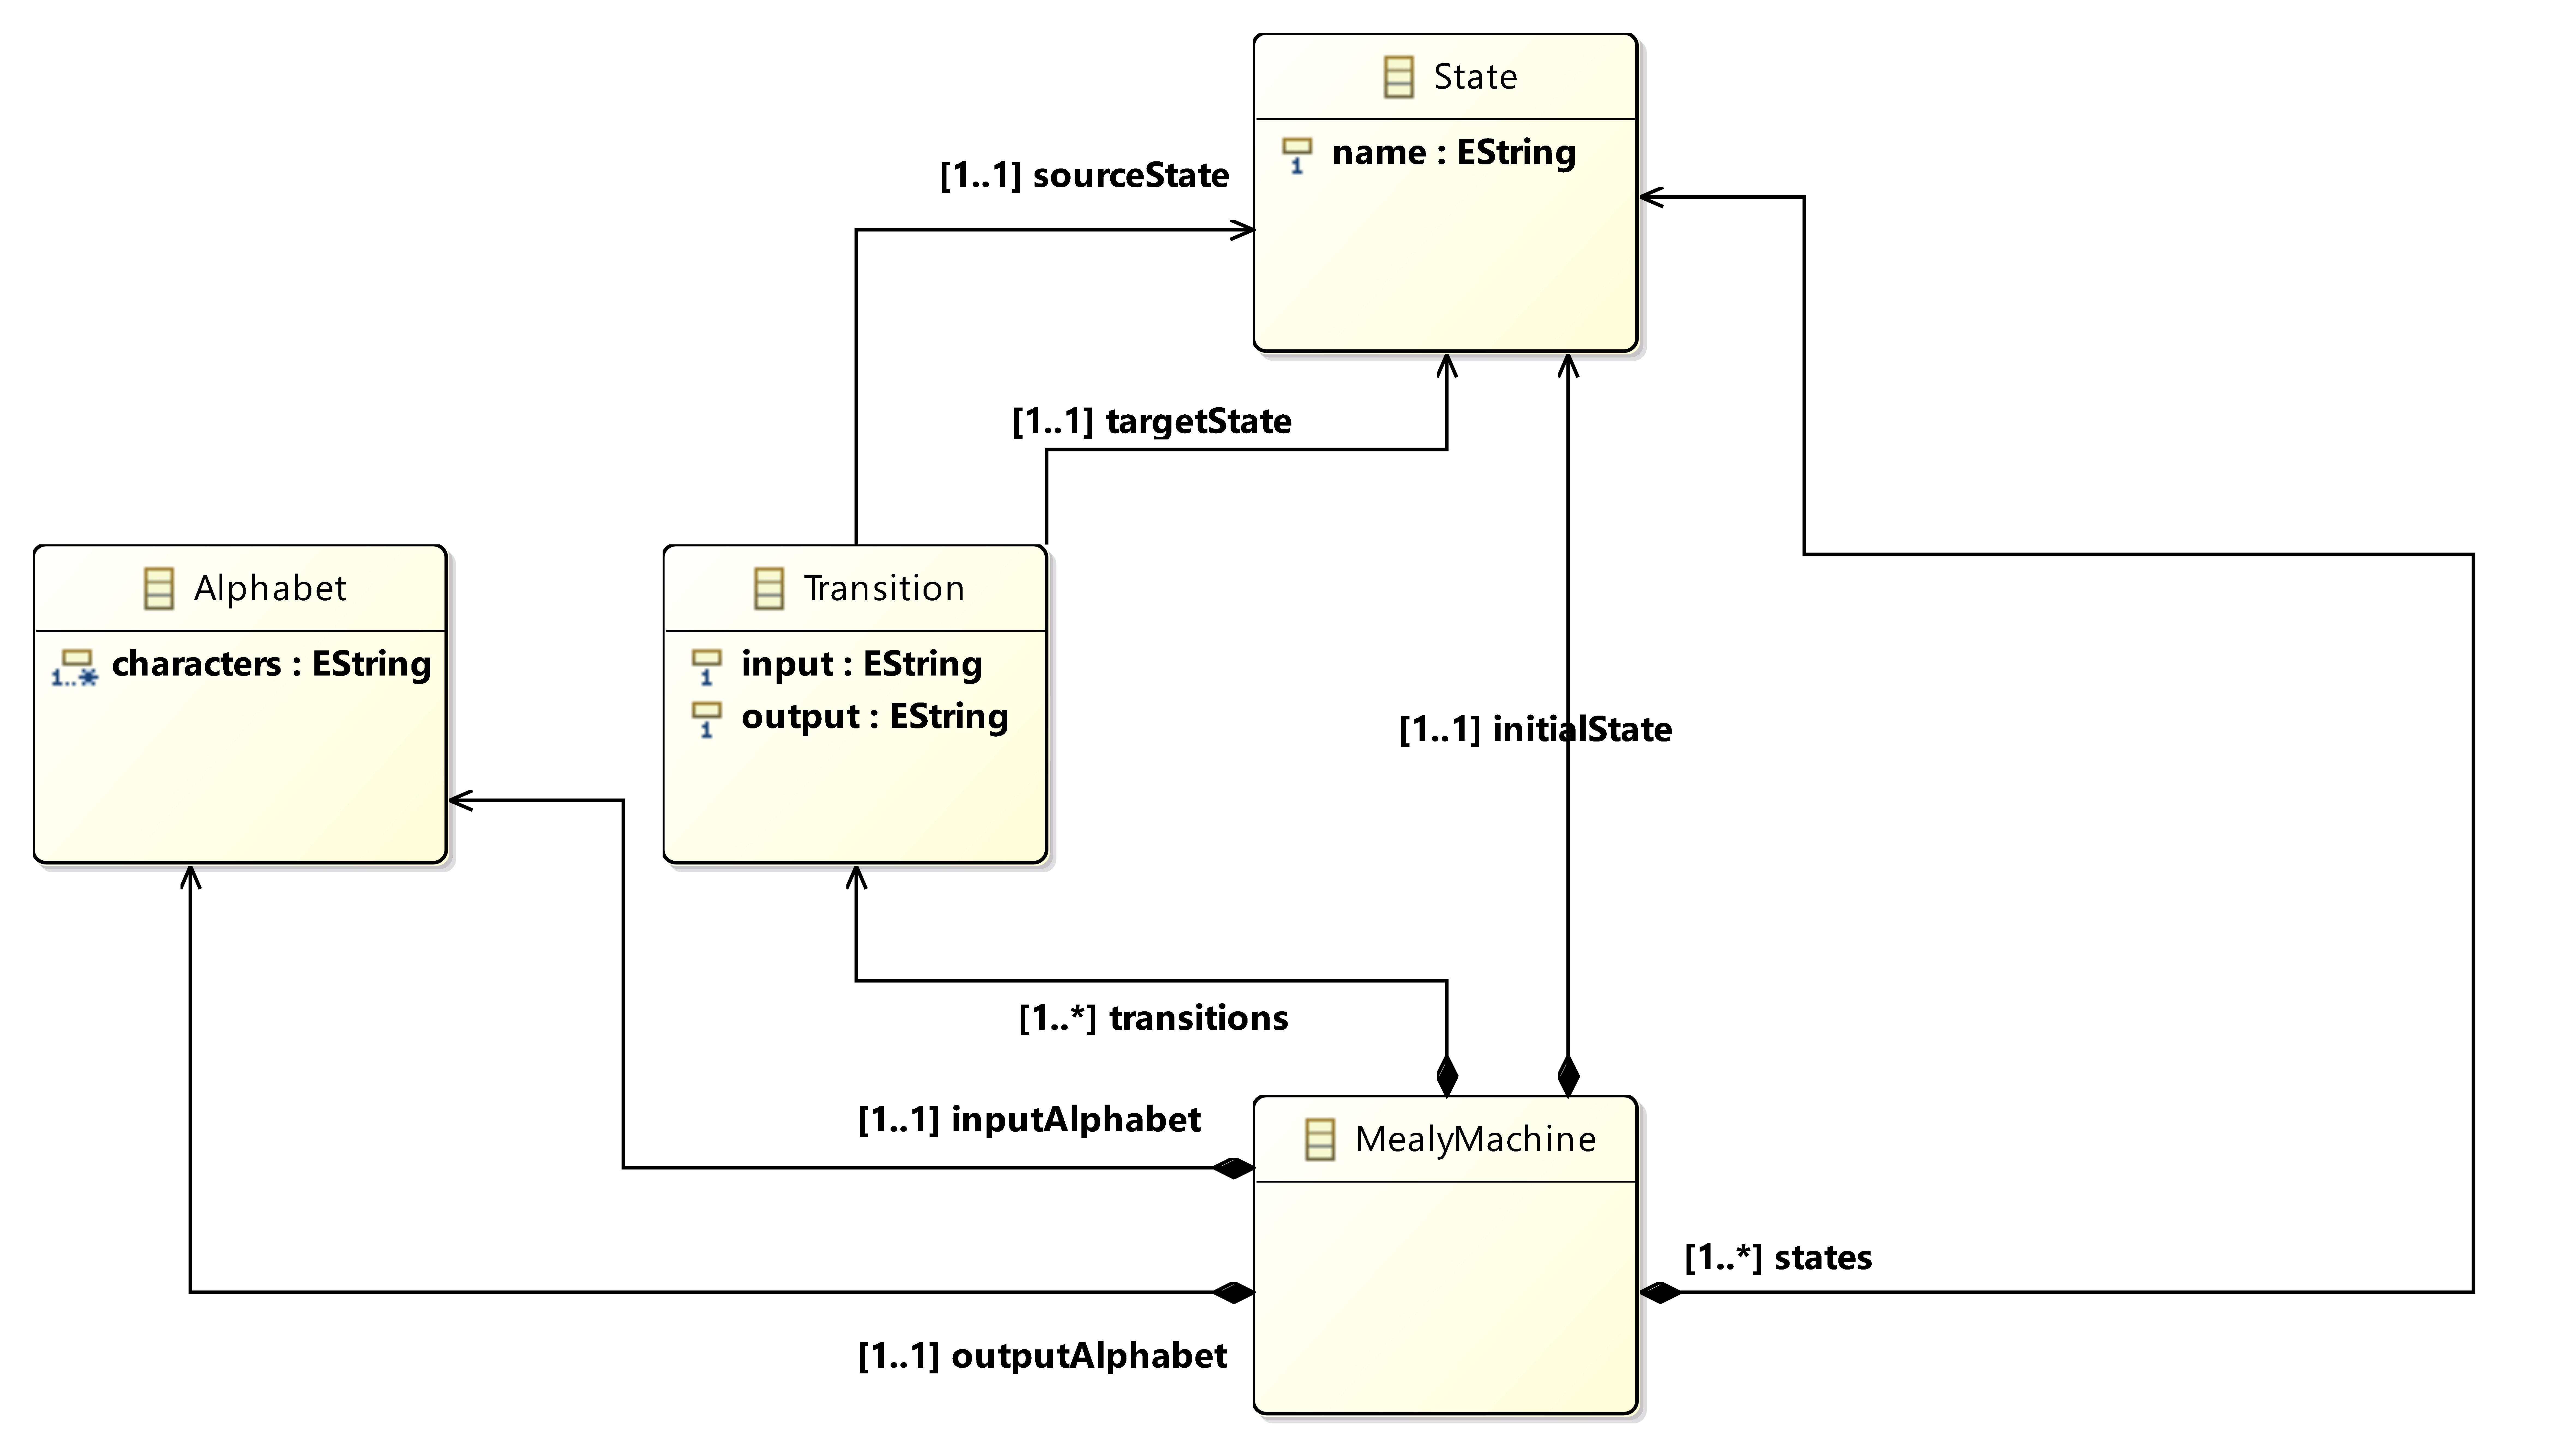
\includegraphics[width=1.0\linewidth]{figures/mealymodel}
	\caption{Ecore metamodel of Mealy machines.}
	\label{fig:mealyecore}
\end{figure}

In text, the Ecore model uses Strings as distinguishers (on code generation, EString is converted to java.lang.String). States of the automaton, i.e. State objects are differentiated based on the name field. Note, that this is a transition-driven model of Mealy machines, the Transition class has a reference to the source and target states of the transition, as opposed to some models, where states store their own transition information (successors, predecessors) like nodes in a graph. This decision was based on the DHC algorithm, which stores traversal information itself, rather than asking for it, which is why ease of access is preferred as opposed to efficiency.

Extending upon the metamodel in Figure \ref*{fig:mealyecore}, I generated the Xtext grammar seen in Listing \ref{li:xtext} utilizing Xtexts EMF integration. In words, this  grammar describes a textual grammar in which instances of the metamodel seen in Fig. \ref{fig:mealyecore} can be stored. 



\begin{lstlisting}[caption=Xtext grammar describing Mealy machines.,label=li:xtext]
MealyMachine returns MealyMachine:
'MealyMachine'
'{'
'initialState' initialState=State
'states' '{' states+=State ( "," states+=State)* '}' 
'inputAlphabet' inputAlphabet=Alphabet
'outputAlphabet' outputAlphabet=Alphabet
'transitions' '{' transitions+=Transition ( "," transitions+=Transition)* '}' 
'}';

State returns State:
{State}
'State'
name=EString;

Alphabet returns Alphabet:
'Alphabet'
'{'
'characters' '{' characters+=EString ( "," characters+=EString)* '}' 
'}';

Transition returns Transition:
'Transition'
'{'
'input' input=EString
'output' output=EString
'sourceState' sourceState=[State|EString]
'targetState' targetState=[State|EString]
'}';

EString returns ecore::EString:
STRING | ID;
\end{lstlisting}

An example of a MealyMachine instance in the form if the grammar in Listing \ref{li:xtext} can be seen in Listing \ref{li:4ixtext}.

\begin{lstlisting}[caption=The Mealy machine seen in Fig.\ref{fig:dfaexamplemealyver}.a in the form of the Xtext grammar described in Listing \ref{li:xtext}.,label=li:4ixtext]
MealyMachine{
initialState 
State q0 states { State q0, State q1, State q2, State q3}
inputAlphabet Alphabet { characters { a , b } }
outputAlphabet Alphabet { characters { top , bot } }
transitions{ 
Transition { input a output top sourceState q0 targetState q1 } , 
Transition { input b output top sourceState q0 targetState q0 } , 
Transition { input a output top sourceState q1 targetState q2 } , 
Transition { input b output top sourceState q1 targetState q1 } , 
Transition { input a output bot sourceState q2 targetState q3 } , 
Transition { input b output top sourceState q2 targetState q2 } , 
Transition { input a output top sourceState q3 targetState q0 } , 
Transition { input b output bot sourceState q3 targetState q3 } } }
\end{lstlisting}

\subsection{Direct Hypothesis Construction}

While implementing the DHC algorithm, I used the above described MealyMachine formalism using the Xtext input source, but I also described a way to programmatically describe an input to ease the process of creating small inputs. An overview of this can be seen in Table \ref{tab:activelearningproto}. Both are expanded upon in the following.

\renewcommand{\tabularxcolumn}[1]{m{#1}}
\newcolumntype{Y}{>{\centering\arraybackslash}X}
\begin{table}[H]
	
	\begin{tabularx}{\columnwidth}{YYYYY}
		\hline
		\textbf{Algorithm} & \textbf{Input formalism} & \textbf{Output formalism} & \textbf{Input source} & \textbf{Output source}\\ \hline
		Direct Hypothesis Construction & Mealy machine & Mealy machine & Xtext & Xtext \\	\hline
		Direct Hypothesis Construction & String sequences & Mealy machine & String & Xtext
		\\ \hline
	\end{tabularx}
	\caption{Overview of the DHC algorithm implementation.}
	\label{tab:activelearningproto}
\end{table}




\label{item:stringsequencelearnable}

The detailed (but not exhaustive) class diagram of the frameworks DHC implementation can be seen in Fig. \ref{fig:abstractdetailedoverview}. The figure is self-explanatory in some regards, while the generic specifics and implementation details are explained in the following.

\begin{itemize}
	\item \textbf{StringSequenceLearnable:} The \emph{StringSequenceLearnable} class is a realization of the Learnable interface, defining simply any type of learnable, which use Strings (java.lang.String) as both input and output types. It contains a simple implementation for describing behavior, accepting a String in the format of $"|input1|output1|input2|output2|...|inputn|outputn|"$, and storing it in a HashMap. One example of this formalism can be seen in Fig. \ref{fig:alternatingbit}.
	
	\item \textbf{MealyLearnable:} The \emph{MealyLearnable} class is a \emph{Learnable} which uses the EMF-modeled \emph{MealyMachine} class seen in Fig. \ref{fig:mealyecore}. Since this implementation of Mealy machines uses Strings as both input and output characters, it extends upon the generic bounds provided by the \emph{StringSequenceLearnable} class.
	
	\item \textbf{DHCHypothesis:} The \emph{DHCHypothesis} abstract class contains the abstractions the DHC algorithm needs to be separated from the implementation of the output formalism. Output here is also implementation-dependent, for DFAs it would be the state after running an input, for Mealy machines it would be output after running an input. Contrary to the \emph{Adapter} layer of input formalisms, every algorithm must define its own abstract hypothesis type, an example being this (the \emph{DHCHypothesis}) class.
	
	\item \textbf{DHCMealyMachineHypothesis:} The \emph{DHCMealyMachineHypothesis} class straightforwardly extends \emph{DHCHypothesis} using the EMF-modeled \emph{MealyMachine} class seen in Fig. \ref{fig:mealyecore}. Essentailly, \emph{DHCMealyMachineHypothesis} is the Mealy machine extension of the DHCHypothesis abstract class, implementing every abstract method of both its superclasses.
	
	\item \textbf{StringSequenceAdapter:} The \emph{StringSequenceAdapter} abstract class adapts \emph{StringSequenceLearnable}s (bounds these using generics), while not defining any generic bounds to the \emph{Hypothesis} it adapts to. This makes it possible to implement equivalance queries only once for every input formalism, using the abstract \emph{convert...()} methods to be implemented by subclasses. The current implementation uses a brute-force method of comparing the outputs of the \emph{Learnable} and the \emph{Hypothesis} for every possible input under the input alphabet. This implementation can be seen in \ref{li:eqbruteforce}.
	
	\item \textbf{StringSequenceToMealyAdapter:} The \emph{StringSequenceToMealyAdapter} class bounds the \emph{Hypothesis} parameters of the \emph{LearnableAdapter} to \emph{DHCMealyMachineHypothesis}, as the dependency relation indicates in Fig. \ref{fig:abstractdetailedoverview}. It only implements the \emph{convert...()} functions.

	\item \textbf{MealyMachineTeacher:} The \emph{MealyMachineTeacher} abstract class bounds the generic parameters of the \emph{Hypothesis} (H) to \emph{DHCMealyMachineHypothesis}, while leaving the \emph{Learnable} (LA) parameter unbound, analogously to \emph{StringSequenceAdapter}. This is done, so algorithm implementations are completely separated from input types. 
	\item \textbf{MealyMachineTeacherStringSequenceImpl:} The \emph{MealyMachineTeacherStringSequenceImpl} class defines the LA generic parameter to be a \emph{StringSequenceAdapter}, and delegates both its methods to it.
	 
	\item \textbf{DirectHypothesisConstruction:} The \emph{DirectHypothesisConstruction} class implements the DHC algorithm using the \emph{DHCHypothesis} abstract class to build its hypothesis. The \emph{constructHypothesis()} method is an implementation of Algorithm \ref{algo:dhc}, constructing a \emph{DHCHypothesis} in a black-box way using the splitters field. The splitters field is initialized and constructed the way described in Algorithm \ref{algo:dhc}, on the first run initialized by the input alphabet, then extended on hypothesis refinement. The \emph{refineHypothesis()} method does exactly this: it takes a counterexample, and adds the suffixes of it to the \emph{splitters}, so the next run of \emph{constructHypothesis()} will split states as needed. The \emph{execute()} method ties everything together by executing \emph{constructHypothesis()}, equivalence queries and the \emph{refineHypothesis()} method. The implementation of the \emph{execute()} method can be seen in Fig. \ref{li:executedhc}.
\end{itemize}

\begin{lstlisting}[caption=The \emph{execute()} function of the DHC algorithm implementation described in Section \ref{item:stringsequencelearnable}s \emph{DirectHypothesisConstruction} item.,label=li:executedhc]
public DHCHypothesis execute() {
	List<? extends I> counterExample = null;
	DHCHypothesis<I, O, M, S, T> h = null;
	do {
		if(counterExample != null) {
			refineHypothesis(counterExample);
		}
		h = constructHypothesis();
		
		counterExample = teacher.equivalenceQuery(h, alphabet);
	}while(counterExample != null);
	
	return h;
}
\end{lstlisting}

Note, that while Table \ref{tab:activelearningproto} states the current working implementations, the algorithm itself runs using its abstract Hypothesis type, resulting in easy extensibility.


\begin{figure}
	\centering
	\vspace*{-1.2cm}
	\hspace*{-1.2cm}
	\centerline{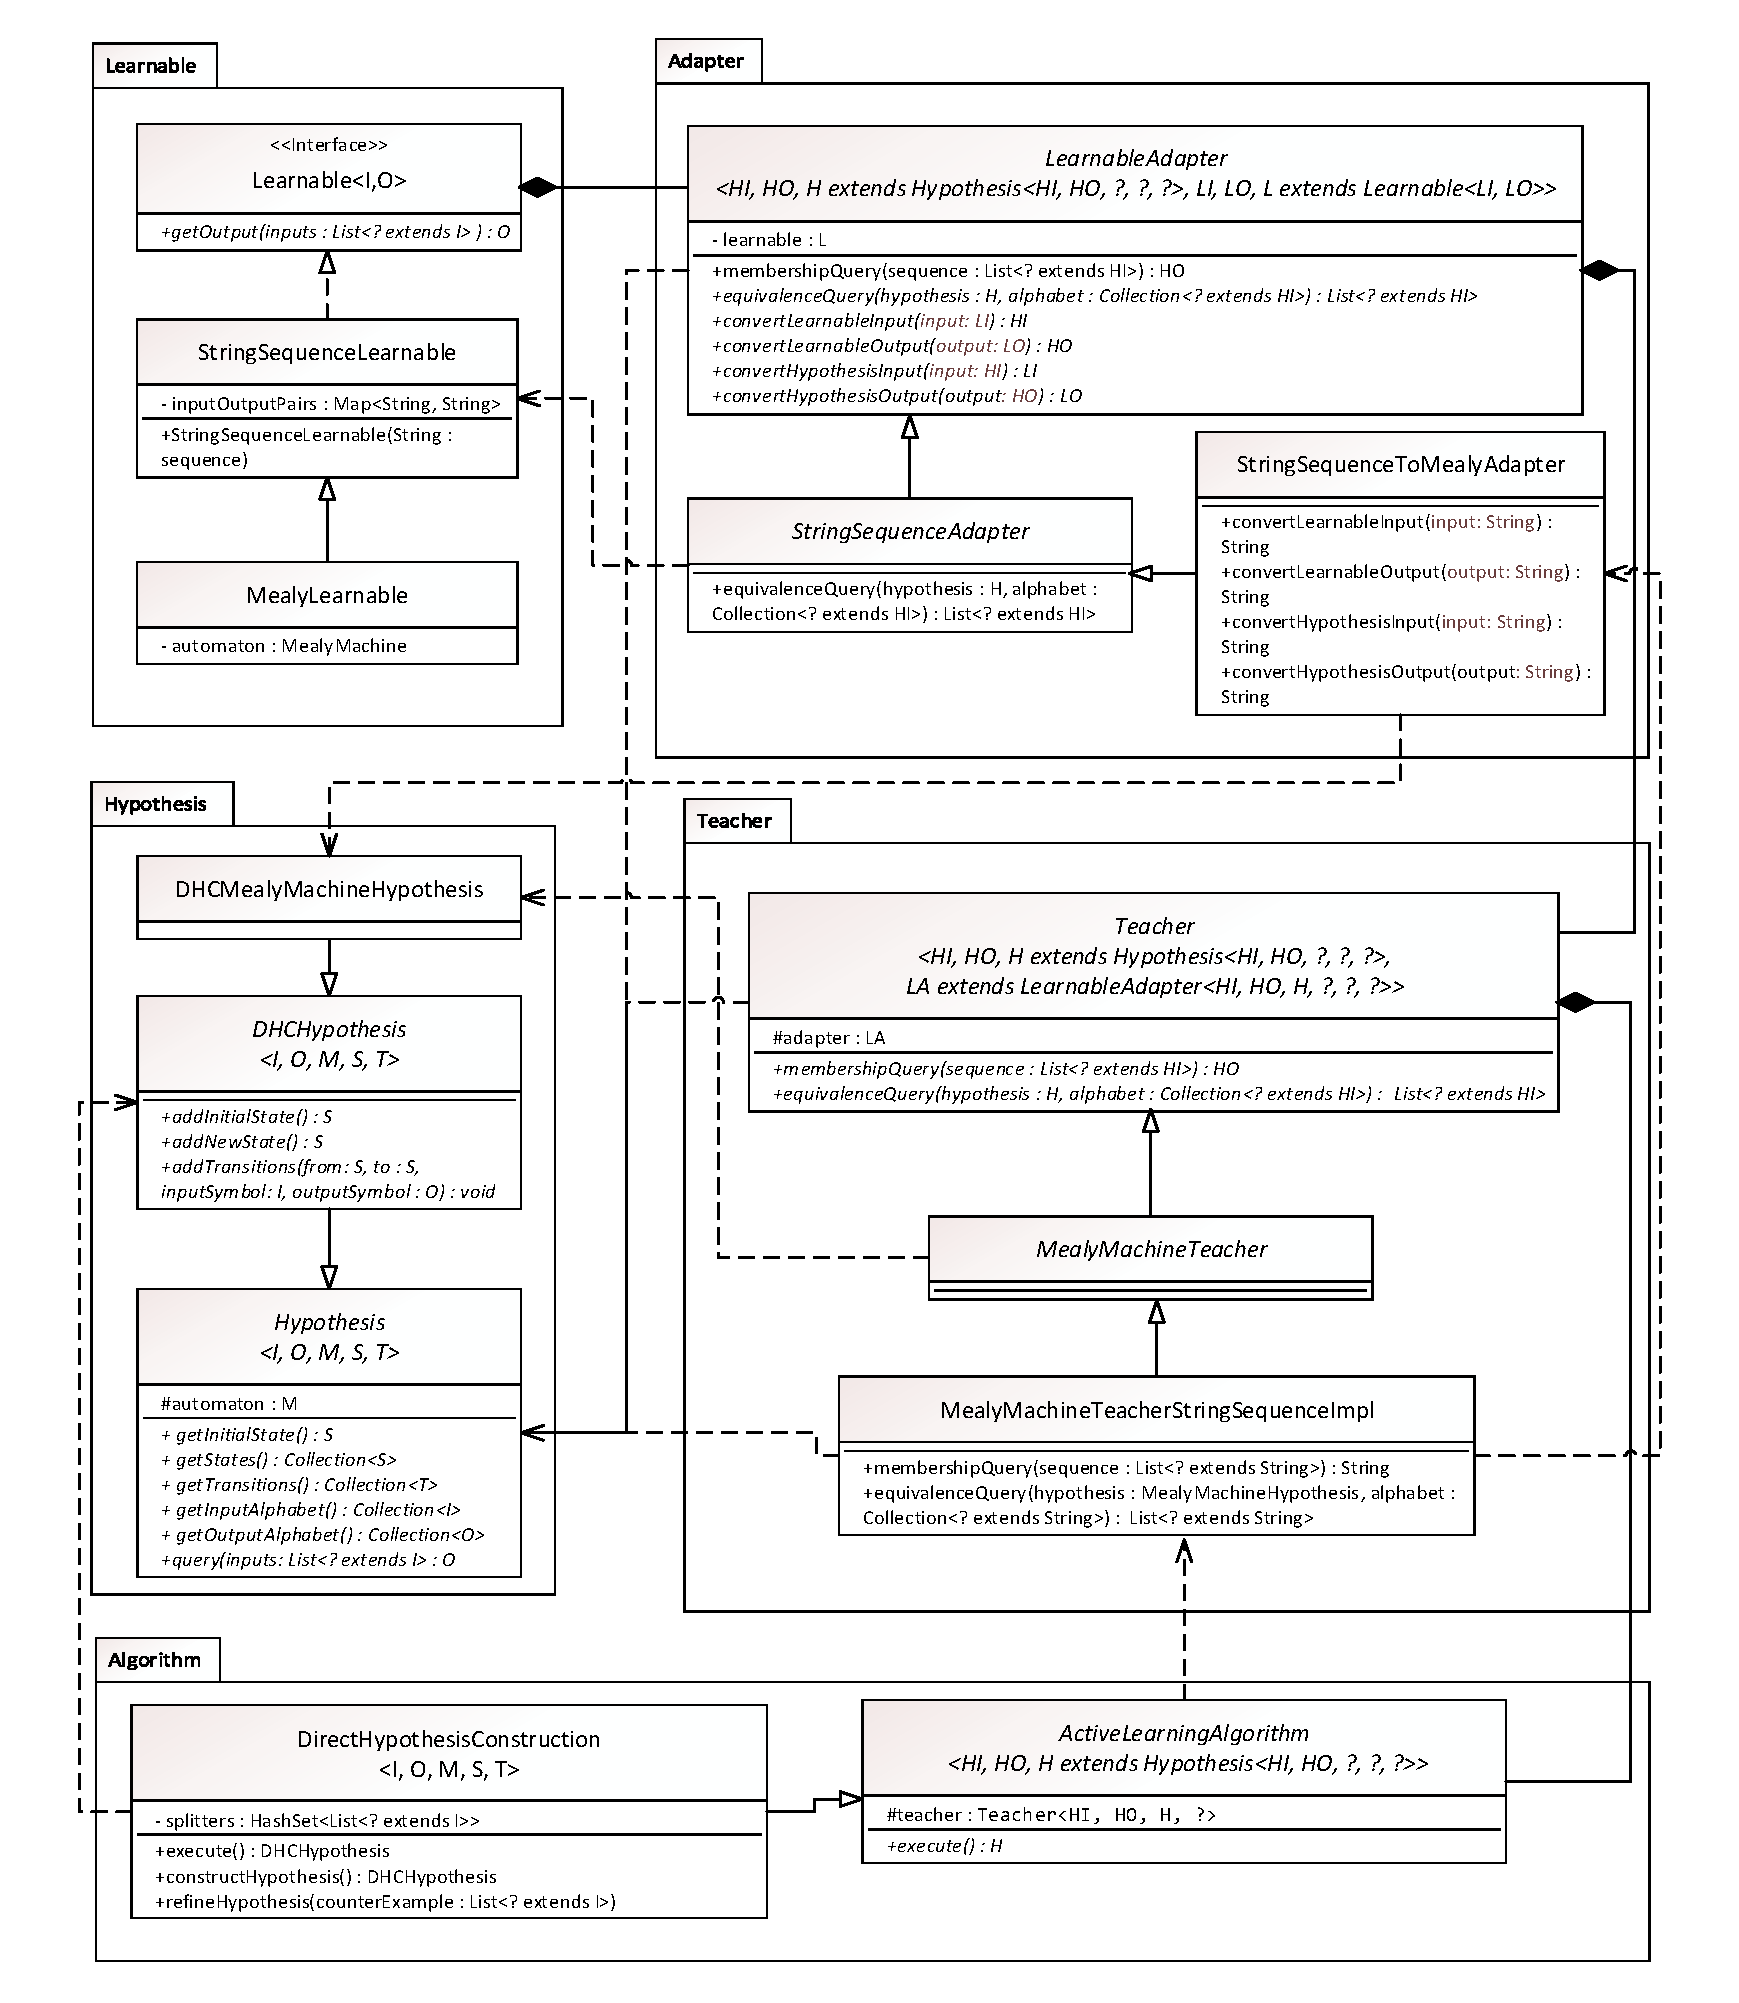
\includegraphics[width=\paperwidth,height=\paperheight,keepaspectratio]{figures/implementationdetailedoverview}}
	\caption{Non-exhaustive detailed structural overview of the frameworks DHC implementation.}
	\label{fig:impldetailedoverview}
\end{figure}

\subsection{TTT}

The TTT algorithm is complex, in both theory and implementation. Due to it using multiple specific types of data structures and sub-algorithms, which are not themselves part of TTT, during my imlementation I depended on the original (defining) implementation of it in LearnLib\cite{10.1007/978-3-319-21690-4_32}.
\\
LearnLib describes an abstract layer of TTT to extend in implementations. I used these abstractions to implement the algorithm into my framework in a (from the perspective of execution) near seamless manner. The current implementation only allows MealyMachines as inputs, but this can be extended upon analogously as with the DHC implementation seen previously.

\renewcommand{\tabularxcolumn}[1]{m{#1}}
\newcolumntype{Y}{>{\centering\arraybackslash}X}
\begin{table}[H]
	
	\begin{tabularx}{\columnwidth}{YYYYY}
		\hline
		\textbf{Algorithm} & \textbf{Input formalism} & \textbf{Output formalism} & \textbf{Input source} & \textbf{Output source}\\ \hline
		TTT & Mealy machine & Mealy machine & Xtext & Xtext \\	\hline
	\end{tabularx}
	\caption{Overview of the TTT algorithm implementation.}
	\label{tab:TTTformalisms}
\end{table}

The implementation itself is built similarly as the DHC implementation, but the algorithm wraps the abstractions of the framework and converts between types of these abstractions and the ones used in LearnLib. More specifically, LearnLib defines abstract types for parts of the TTT algorithms, such as \emph{AbstractTTTHypothesis},\emph{AbstractBaseDTNode} (abstract discriminator tree node), \emph{AbstractTTTLearner}. While LearnLib has implementations of these, I only depended on abstractions, using the current implementation as reference.
\\\\
For key steps of TTT, the responsibilities of the current implementation are as follows. The Hypothesis construction and refinement is done by my framework, which provides the methods of hypothesis construction, while also hadling the calculation of output inconsistencies and the refinement of them. LearnLib manages the internal data structures including the dicriminator tree, which stores my implementation of the $AbstractBaseDTNode$ class. The state splitting (part of Hypothesis stabilization) and discriminator finalization is handled by LearnLib.
